\chapter{System Under Consideration} \label{ch:system}
The following chapter gives a thorough explanation of the system under consideration of this thesis. The system in question is the \textit{SecuritasHome startpaket}, which is a home alarm system from SecuritasHome. This starter-kit includes multiple hardware components, as well as access to software portals and mobile applications to control the system.

\section{Components and Software} \label{ch:system:components}
This section describes all the components and software of the system. Initially, all hardware components are described and their functionality. Lastly, all software components of the system are described. Note that the system supports many additional hardware components. The ones listed below are the ones part of the starter-kit.

While the system was sold by SecuritasHome, they have little to do with the actual hardware and software components of the platform, see figure \ref{fig:company-structure}. The hardware, related firmware, and radio wave protocol are manufactured by a Taiwanese company called \textit{Climax Technology}. The software like the web portal and mobile applications as well as some additional firmware are made by an American company called \textit{Alarm.com}. SecuritasHome merely sell and advertise the product and put their brand on it. Their main contribution to the system is in terms of real-time response to an alarm, connection to an alarm-central, and sending security personnel to respond to an active alarm breach.
\begin{figure}[!ht]
  \begin{center}
    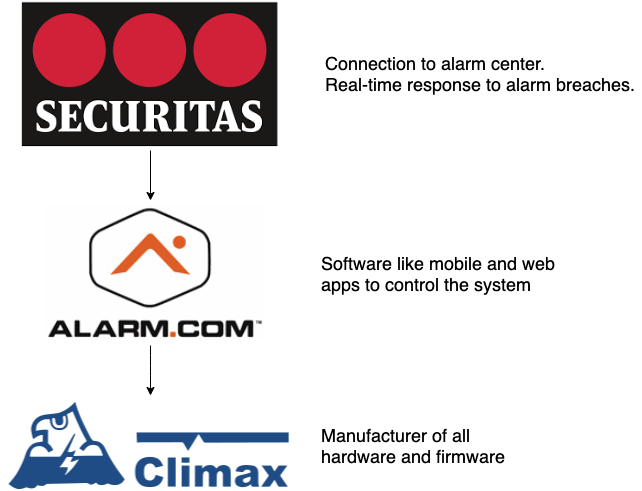
\includegraphics[width=0.5\textwidth]{images/company-structure.png}
  \end{center}
  \caption{The companies behind the system.}
  \label{fig:company-structure}
\end{figure}

\subsection{Hardware components} \label{ch:system:hardware}
\subsubsection{Main Panel}
\textbf{Model number:} HSGW-G8-3G/LTE-ZW-F1 433/868 \\
\textbf{FCCID:} GX9HSGWF1919 \\
The main panel is the \textit{"brains"} of the system so to speak. See figure \ref{fig:main-panel}. It handles communication with all other hardware devices as well as external servers. This is a \texttt{HSGW-G8} from Climax Technology. Through radio wave communication it talks to the other hardware peripherals of the system. It uses 3G telecommunication to talk to the external servers.
\begin{figure}[!ht]
  \begin{center}
    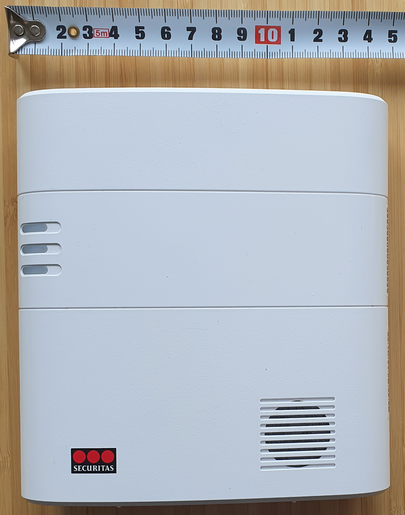
\includegraphics[width=0.5\textwidth]{images/main-panel.png}
  \end{center}
  \caption{Main Panel}
  \label{fig:main-panel}
\end{figure}

\subsubsection{Remote Keypad}
\textbf{Model number:} KPT-23-EL-F1 \\ % could also be KPT-23N-EL-F1, not sure
\textbf{FCCID:} GX9KPF1 \\ % This says KPF but it looks the same..
The remote keypad is a 16 button keypad used to arm the system using a personal 4 digit pin. See figure \ref{fig:remote-keypad}. This device talks to the main panel over radiowave communication.
\begin{figure}[!ht]
  \begin{center}
    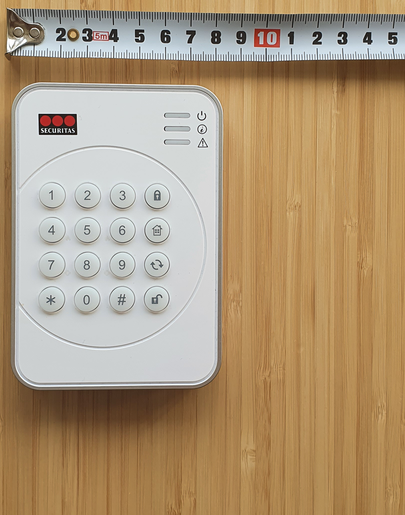
\includegraphics[width=0.5\textwidth]{images/keypad.png}
  \end{center}
  \caption{Remote keypad}
  \label{fig:remote-keypad}
\end{figure}

\subsubsection{Motion Detection Camera}
\textbf{Model number:} VST-862-F1 \\
\textbf{FCCID:} GX9862 \\
This device, see figure \ref{fig:motion-camera}, features an infra-red sensor to detect motion, and a camera to survey the location. When triggered the devices takes two pictures which are sent to the main panel. It is not a surveillance camera, meaning it does not continuously take pictures. This is only done when motion is detected, presumably to save power.
\begin{figure}[!ht]
  \begin{center}
    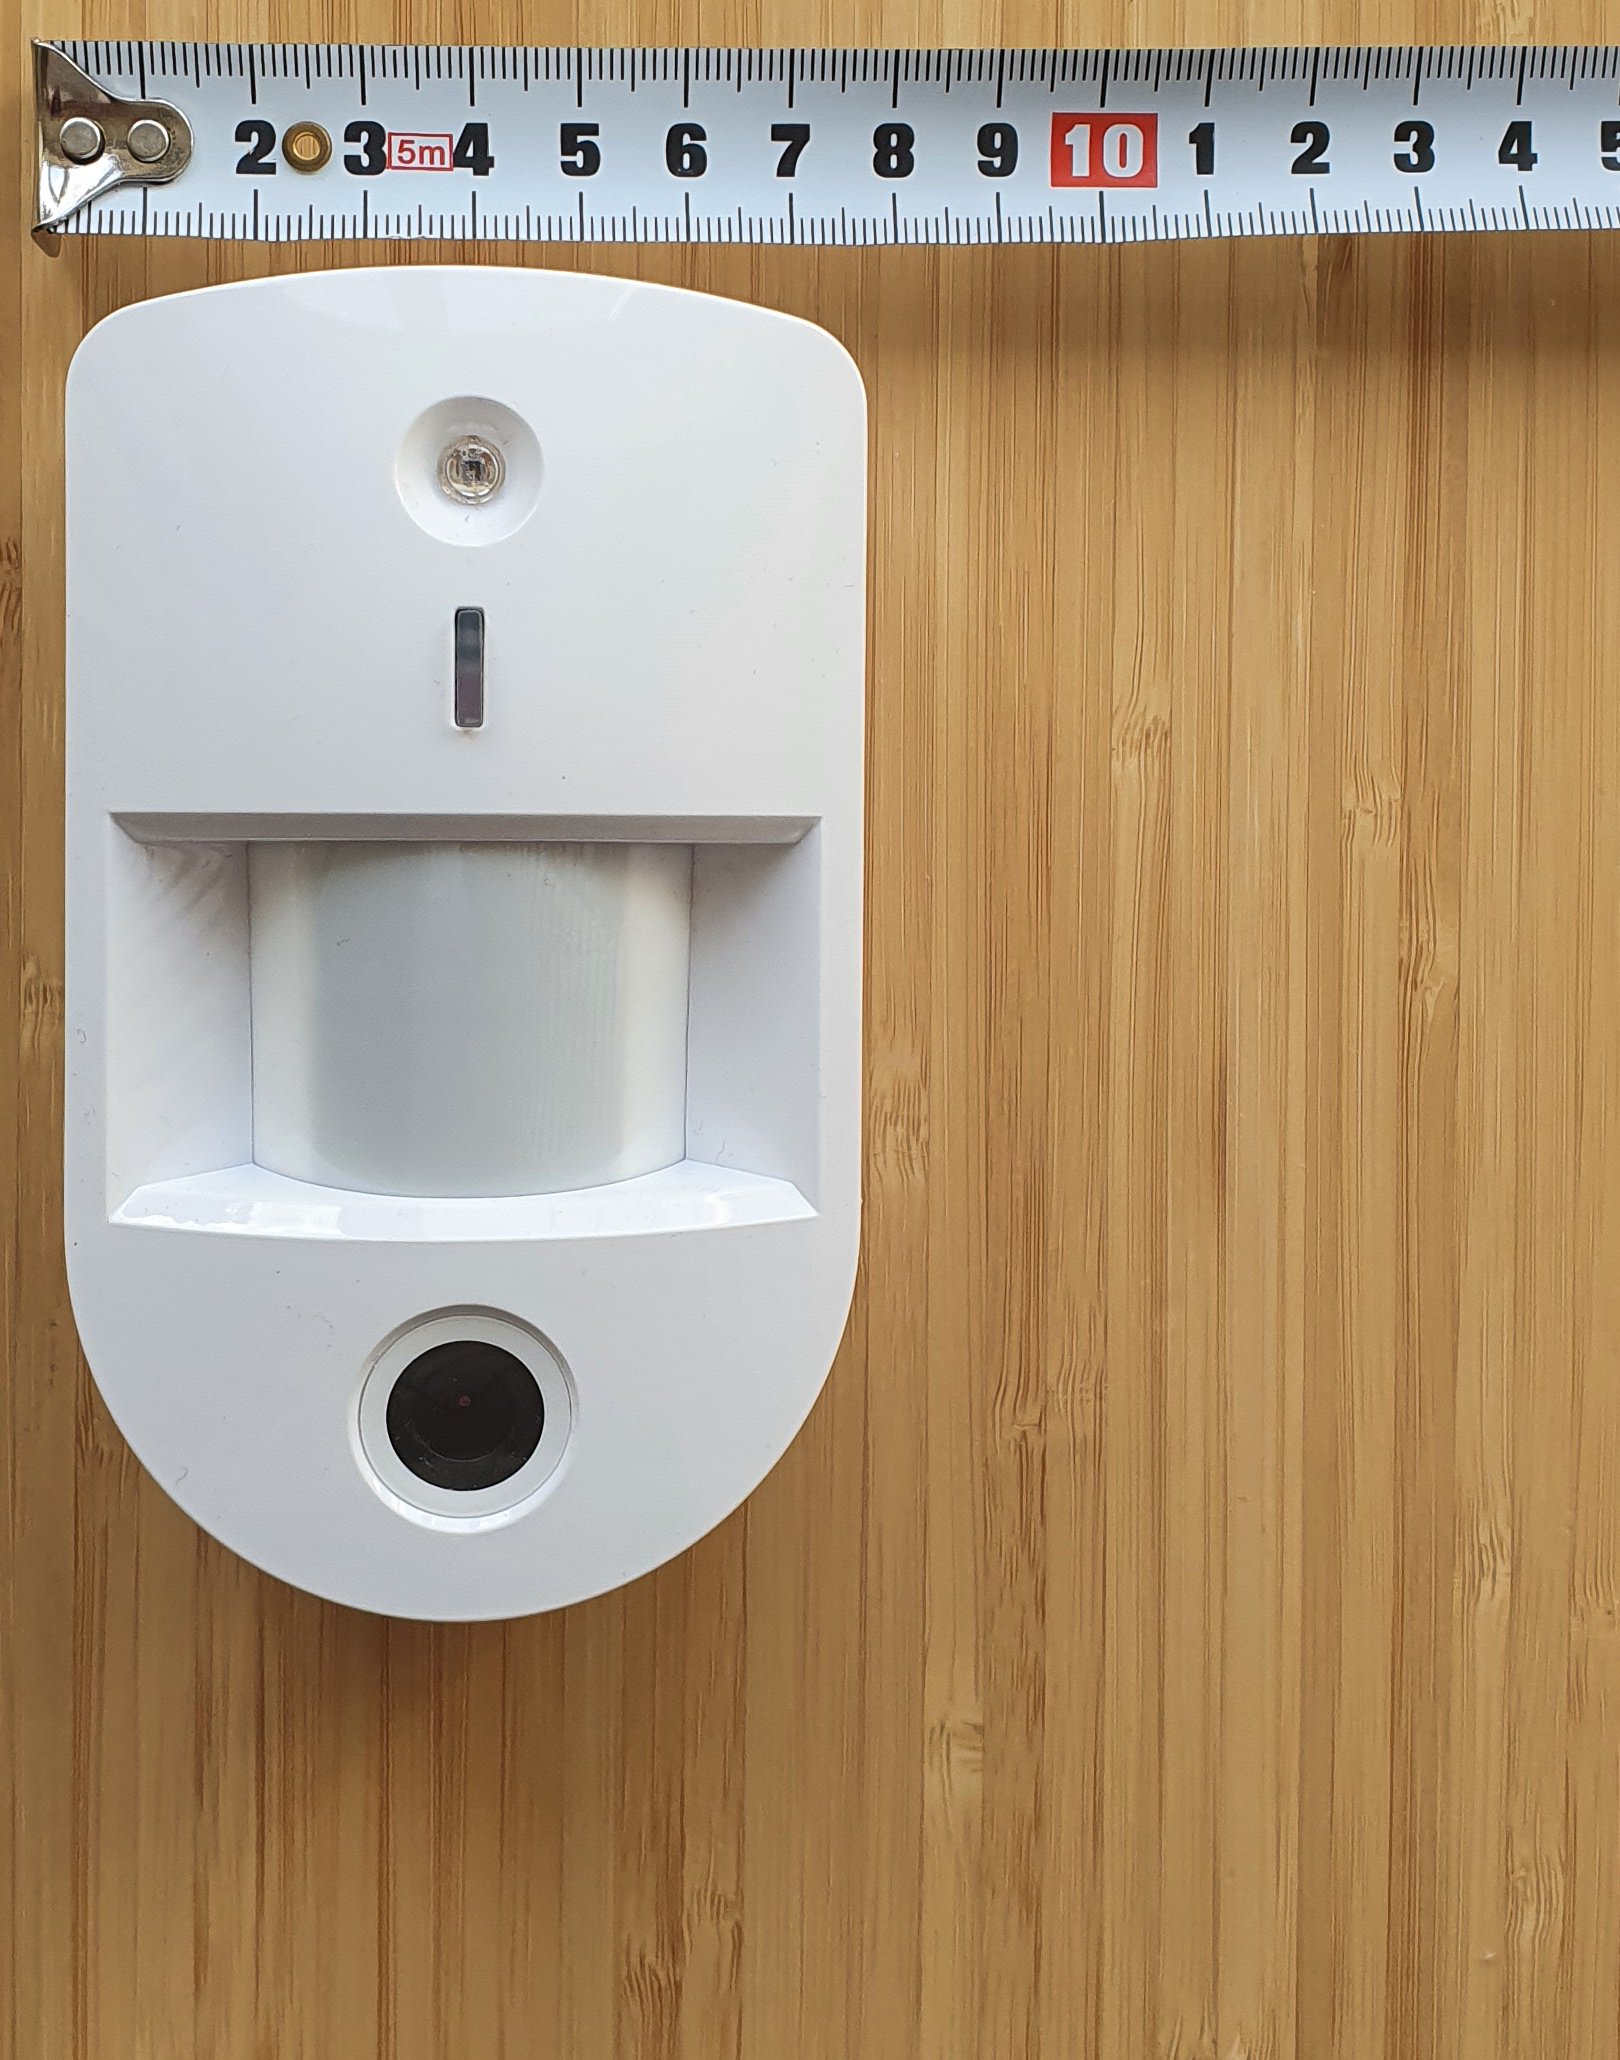
\includegraphics[width=0.5\textwidth]{images/camera.png}
  \end{center}
  \caption{Motion Detection Camera}
  \label{fig:motion-camera}
\end{figure}

\subsubsection{Door Contact Sensor}
\textbf{Model number:} DC-23-F1 \\
\textbf{FCCID:} GX9DC23 \\
This device, see figure \ref{fig:door-contact}, senses when a door or window is opened. A small external magnet is placed on the door/window close to the device. When these are separated the device is triggered and communicates with the main panel over radio waves.
\begin{figure}[!ht]
  \begin{center}
    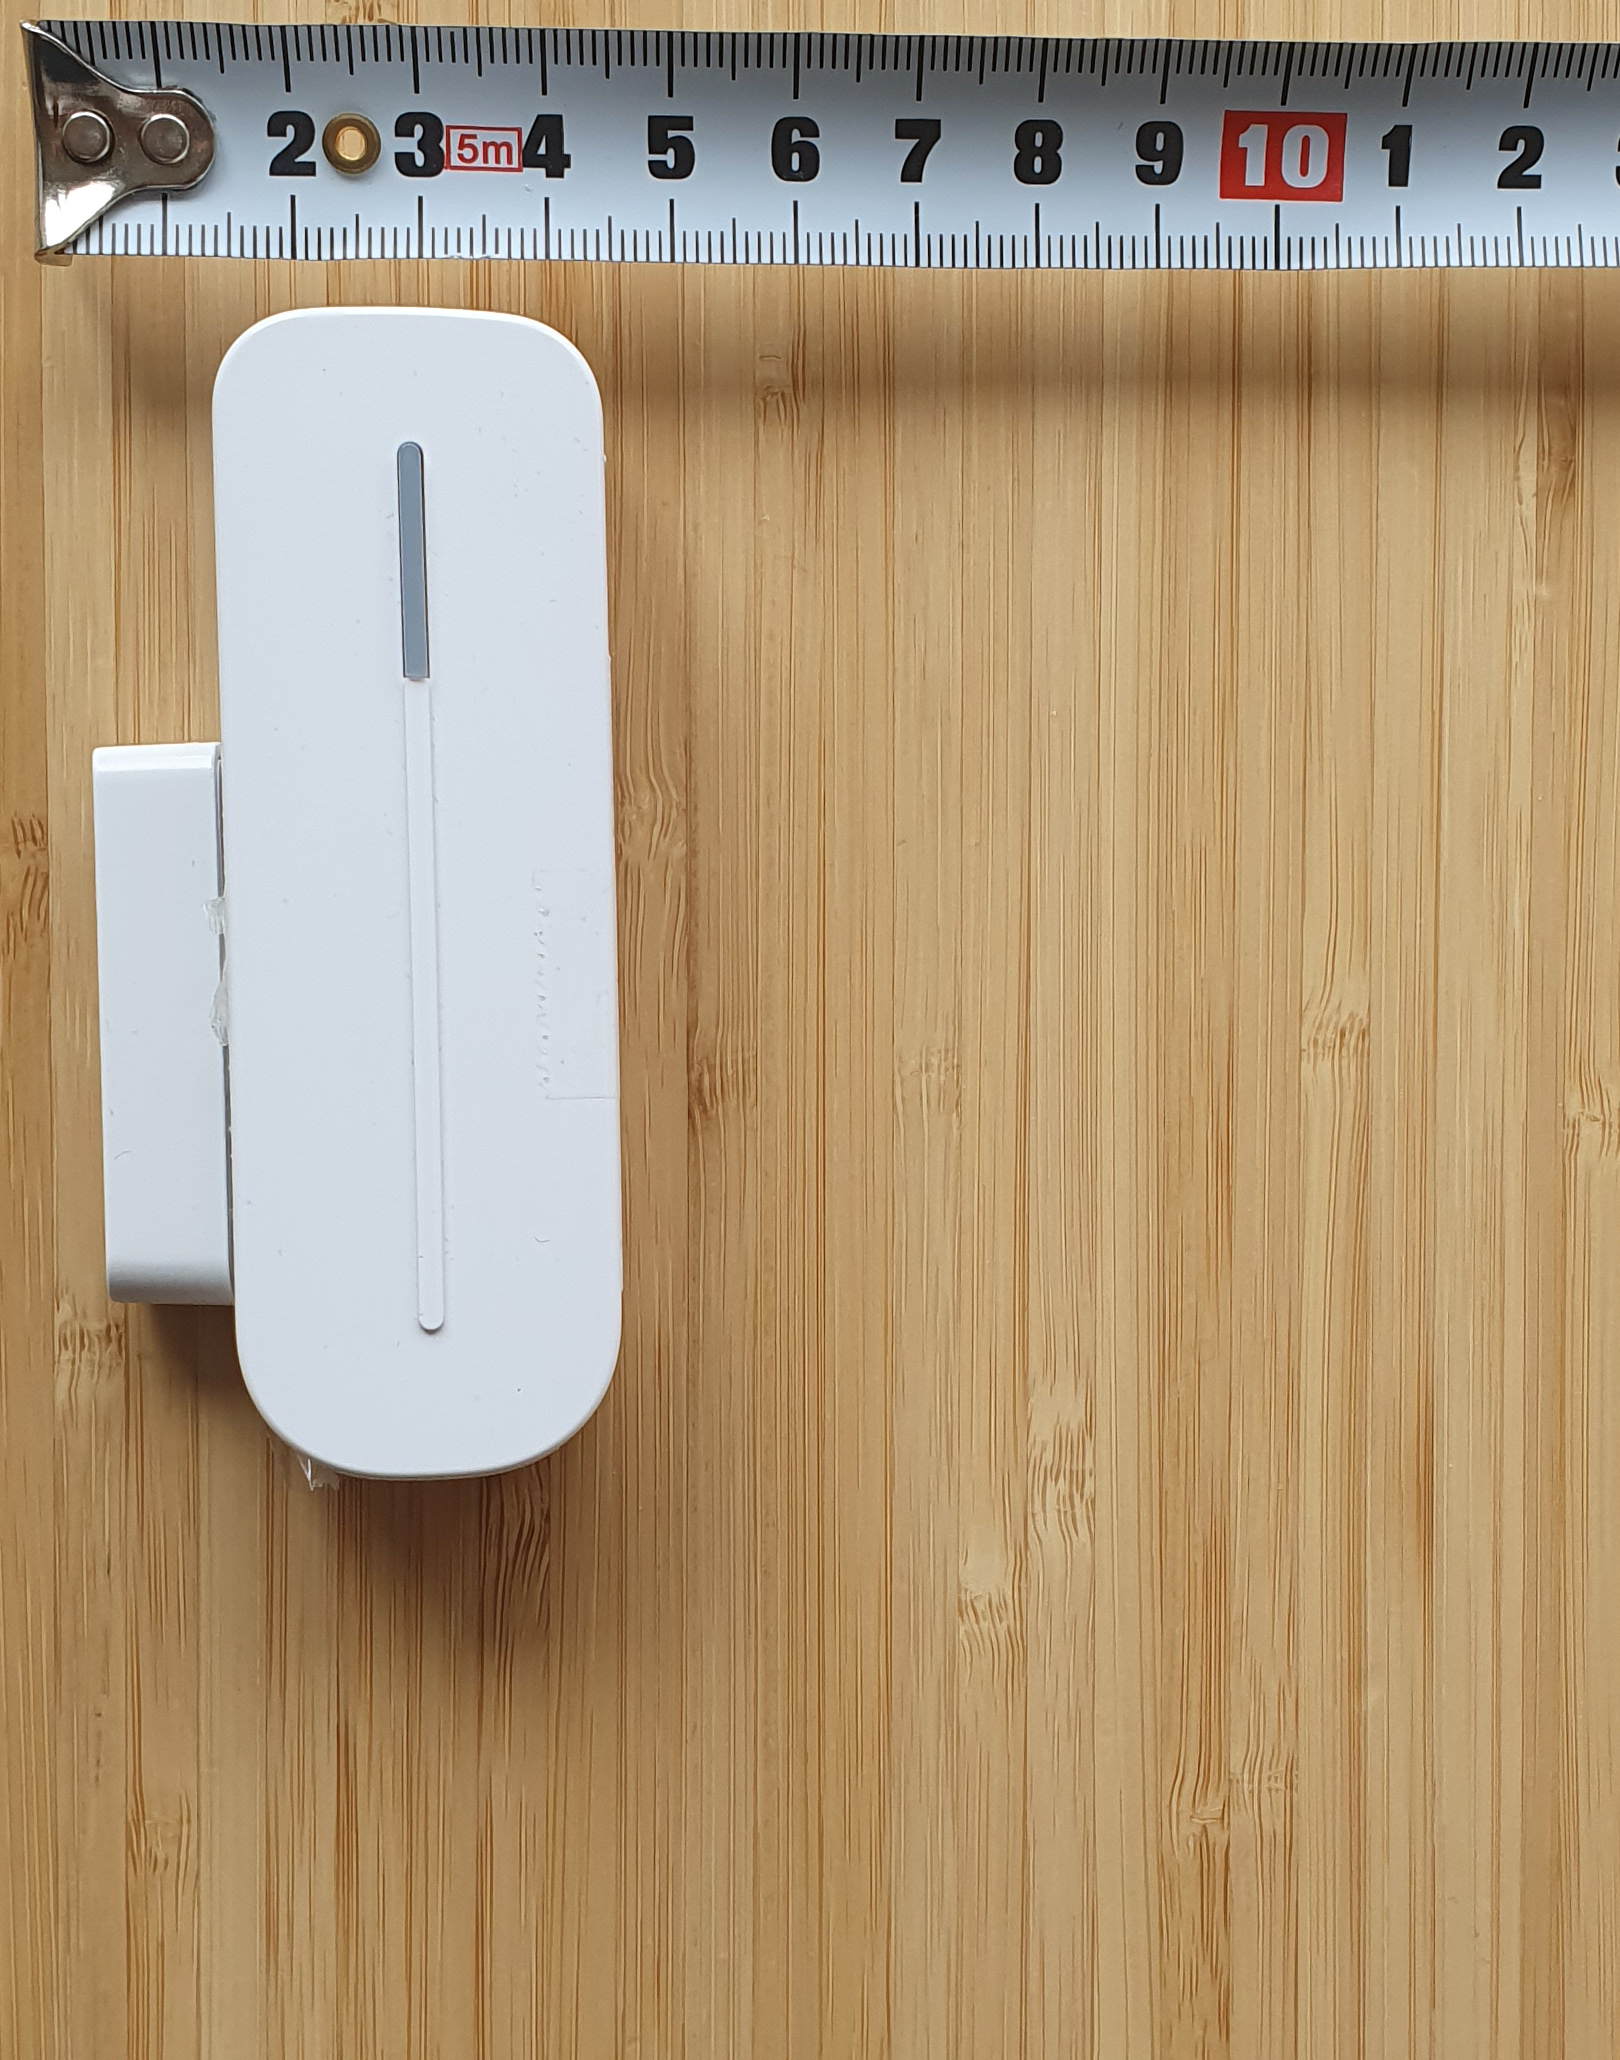
\includegraphics[width=0.5\textwidth]{images/door-contact.png}
  \end{center}
  \caption{Door Contact Sensor}
  \label{fig:door-contact}
\end{figure}

\subsubsection{Smoke Detector}
\textbf{Model number:} SD-8EL \\
\textbf{FCCID:} GX9SD8ELF1919 \\
This device is a smoke detector, see figure \ref{fig:smoke-detector}. It communicated with the main panel over radio-waves and also includes a siren which triggers when it detects smoke.
\begin{figure}[!ht]
  \begin{center}
    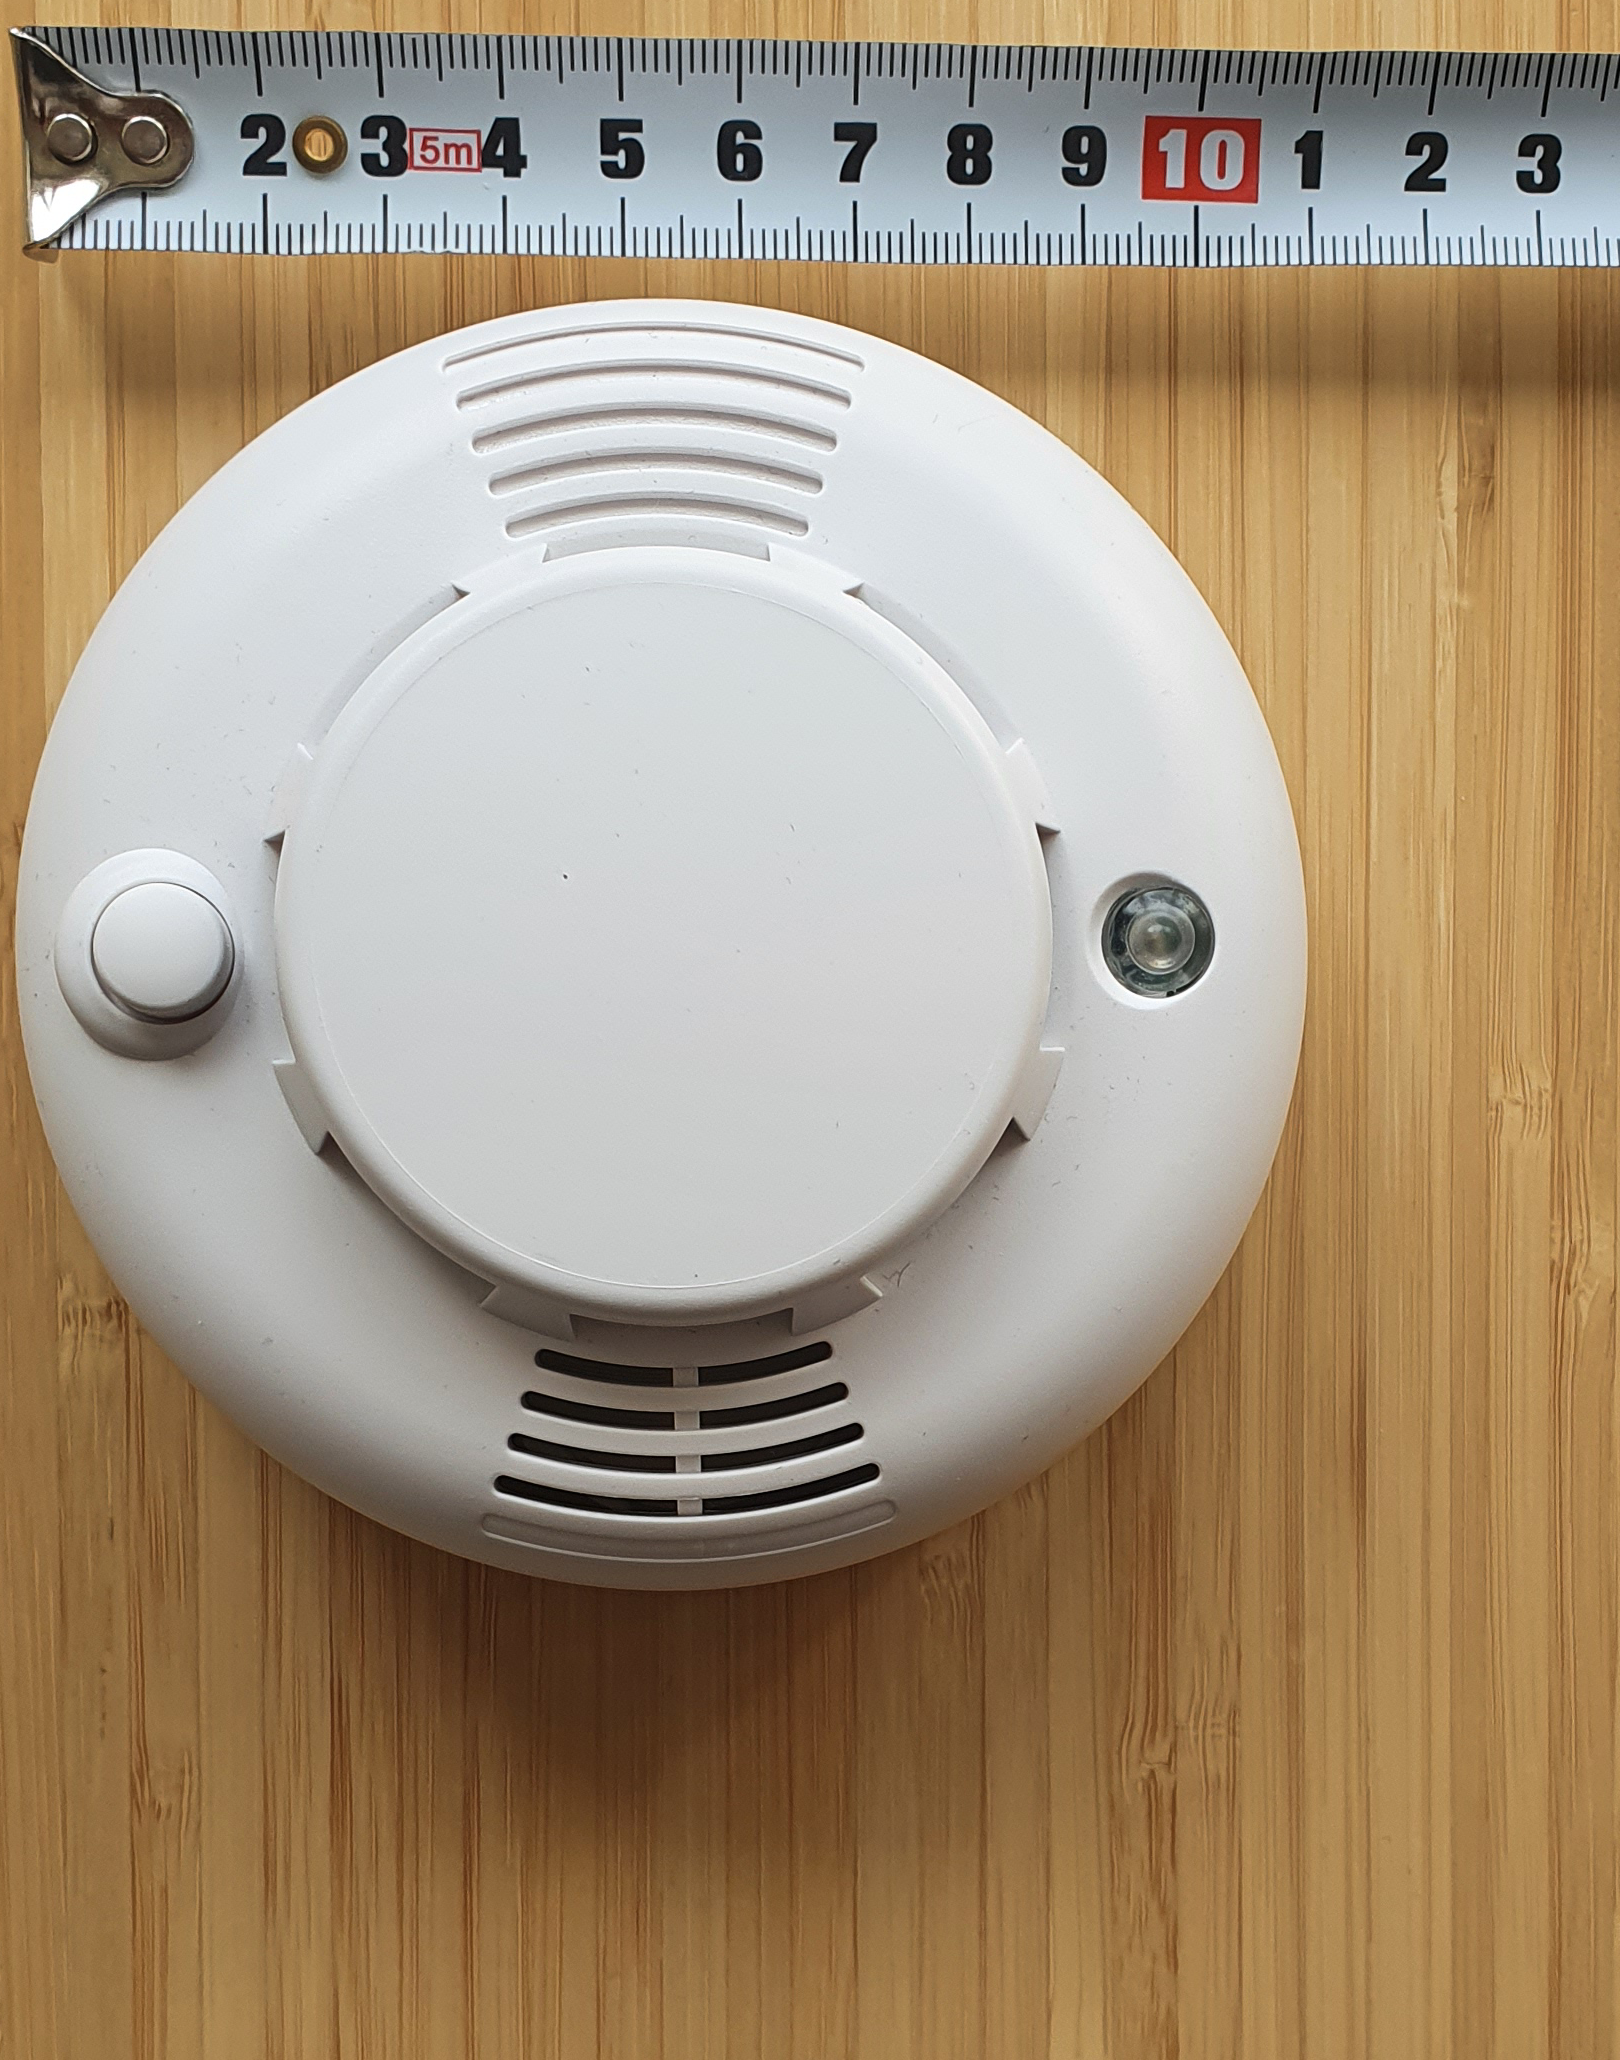
\includegraphics[width=0.5\textwidth]{images/smoke-detector.png}
  \end{center}
  \caption{Smoke Detector}
  \label{fig:smoke-detector}
\end{figure}

\subsection{Software} \label{ch:system:software}
\subsubsection{Web portal}

\subsubsection{Mobile application}

\subsubsection{Local web admin page}